\section{Theorie}
\label{sec:theorie}

    Im folgenden Abschnitt werden die theoretischen Grundlagen eines Lasers (light amplification by stimulated emission of radiation) beschrieben.

\subsection{Bestandteile und Funktionsweise eines Lasers}

    Ein Laser besteht im Wesentlichen aus drei Bestandteilen:
    dem aktiven Medium, einer Energiepumpe und einem Resonator.
    Auf den Resonator wird in \autoref{sec:stabilitaet} näher eingegangen.
    In einem Laserrohr sind aktives Medium und Energiepumpe zusammengefasst,
    welche meist durch zwei Gase realisiert sind.
    Mithilfe der Energiepumpe sollen die Atome des aktiven Mediums durch Stöße angeregt werden,
    sodass sich eine sogenannte \textit{Besetzungsinversion} einstellt.
    Damit ist gemeint,
    dass sich im aktiven Medium mehr Elektronen auf einem höheren Energieniveau als auf einem niedrigeren befinden.
    Mithilfe von spontaner oder stimulierter Emission,
    welche in \autoref{fig:absorption_emission} dargestellt sind,
    fallen die Elektronen wieder auf das niedrigere Energieniveau zurück
    und die Energiedifferenz wird in Form eines Photons mit der entsprechenden Wellenlänge frei.
    Je größer die Besetzungsinversion ist,
    je mehr Elektronen sich also auf einem höheren Niveau befinden,
    desto größer ist die Verstärkung des Laserlichts,
    da mehr Elektronen in den niedrigeren Zustand zurückkehren.
    \begin{figure}[H]
       \centering
       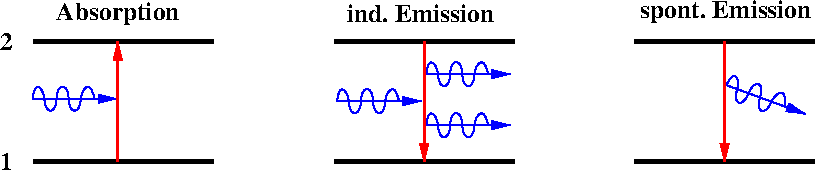
\includegraphics[width=\textwidth]{content/img/Altanleitung/Abb_1_edit.pdf}
       \caption{Schematische Darstellung von Absorption, spontaner und stimulierter (\textit{ind.}) Emission in einem Zwei-Niveau-System.}
       \label{fig:absorption_emission}
    \end{figure}
    Aufgrund der Maxwell-verteilten Besetzung der Elektronen in einem Zwei-Niveau-System kann in diesem System keine Besetzungsinversion erreicht werden;
    für einen Laser sind also mehr als zwei Niveaus erforderlich.\\
    \\
    Im Falle des He-Ne-Lasers wird das aktive Medium durch Neon realisiert,
    die Energiepumpe durch Helium-Atome,
    welche zu Beginn durch Stöße mit Elektronen angeregt werden und die überschüssige Energie bei einem Stoß zweiter Art an die Neon-Atome übertragen.
    Der He-Ne-Laser ist ein Drei-Niveau-Laser,
    es werden die oberen $2s$- und $3s$-Niveaus im Neon besetzt.
    Aufgrund der Auswahlregel $\symup{\Delta} l = \pm 1$ können nur Übergänge in niedrigere $p$-Niveaus stattfinden.
    Der hier beobachtete Übergang $3s_2 \to 2p_4$ entspricht einer roten Linie mit der Wellenlänge $\lambda = \SI{632.816}{\nano\meter}$.

\subsection{Stabilität der Resonatoren}
\label{sec:stabilitaet}

    Der Resonator besteht aus zwei semipermeablen Spiegeln und umgibt das Laserrohr,
    in dem sich aktives Medium und Energiepumpe befinden.
    Aufgrund der Beschaffenheit der Spiegel wird ein Teil des entstehenden Lichts reflektiert,
    während der andere Teil durch die Spiegel hindurch geht.
    Er dient dazu,
    das emittierte Licht zu reflektieren,
    sodass sich zwischen den Resonatorspiegeln eine stehende Welle ausbildet.
    Der Resonator soll aufgrunddessen einen selbstschwingenden Oszillator bilden,
    da das Licht der stehenden Welle wieder auf die Neon-Atome trifft und so selbst wieder Atome anregt.
    Dieses Phänomen wird Absorption genannt und ist ebenfalls in \autoref{fig:absorption_emission} dargestellt.\\
    Damit der Resonator eine stehende Welle ausbilden kann,
    also stabil ist,
    muss die \textit{Stabilitätsbedingung}
    \begin{equation}
        0 < g_i \cdot g_j < 1
        \label{eqn:stabilitaetsbedingung}
    \end{equation}
    erfüllt sein.
    Die Parameter $g_i, g_j$ werden mithilfe von
    \begin{equation}
        g = 1 - \frac{L}{r_i}
        \label{eqn:stabilitaetsparameter}
    \end{equation}
    berechnet,
    wobei $L$ die Resonatorlänge und $r_i$ der Radius des verwendeten Spiegels ist.
    Für zwei plane Spiegel mit dem Radius $r = \infty$ wäre das Produkt $g_ig_j = 1$ und der Resonator damit metastabil.
    Auch in diesem Fall kann der Laser trotzdem funktionieren.
    Für die hier verwendeten Resonatoren,
    bestehend aus zwei konkaven Spiegeln mit Radius $r = \SI{1400}{\milli\meter}$ im ersten Fall und einem planen und einem konkaven Spiegel mit Radius $r = \SI{1400}{\milli\meter}$ im zweiten Fall,
    ergibt sich nach \autoref{eqn:stabilitaetsbedingung} im ersten Fall eine maximale Länge von $L_\text{konkav,konkav} = \SI{2800}{\milli\meter}$ und im zweiten Fall $L_\text{plan,konkav} = \SI{1400}{\milli\meter}$.
    Der Verlauf der Stabilitätsbedingung $g_i \cdot g_j$ als Funktion der Resonatorlänge $L$ ist in \autoref{fig:plt:stabilitaetsbedingung_theorie} für verschiedene Kombinationen von Spiegeln dargestellt.
    \begin{figure}[H]
        \centering
        \includegraphics[width=\textwidth]{build/plt/2_stabilitaetsbedingung_theorie.pdf}
        \caption{Stabilitätsparameter $g_1 \cdot g_2$ in Abhängigkeit der Resonatorlänge $L$ für verschiedene Spiegelkonfigurationen.}
        \label{fig:plt:stabilitaetsbedingung_theorie}
    \end{figure}


\subsection{Transversale und longitudinale Moden in einem Laser}
\label{sec:moden}

    In einem offenen Resonator bildet sich eine stehende Welle aus,
    die aus longitudinalen und transversalen Moden besteht.
    Longitudinale Moden sind dabei längs der Ausbreitungsrichtung,
    die transversalen Moden senkrecht zur Ausbreitungsrichtung.
    Die transversalen Moden werden auch \TEM{mn}-Moden genannt,
    \enquote{Transversal electromagnetic}.
    Der Index $mn$ bezeichnet die Anzahl der Knoten in der hier $xy$-Ebene.\\
    In diesem Versuch sollen die \TEM{00}- und die \TEM{01}-Mode untersucht werden.
    Die \TEM{00}-Mode wird auch als \textit{Fundamentalmode} bezeichnet.
    Ihre Intensitätsverteilung hat die Form einer (zweidimensionalen) Gauß-Kurve,
    wie in \autoref{fig:theorie:tem_00} erkennbar ist.
    Die Intensitätsverteilung der \TEM{01}-Mode ist in \autoref{fig:theorie:tem_01} dargestellt.

    \begin{figure}
    \centering
    \begin{subfigure}{.5\textwidth}
        \centering
        \includegraphics[width=.5\linewidth]{build/plt/tem_00.png}
        \caption{\TEM{00}}
        \label{fig:theorie:tem_00}
    \end{subfigure}%
    \begin{subfigure}{.5\textwidth}
        \centering
        % Ja, wirklich 10, nicht 01. So stimmt es mit Wikipedia und unserer Beobachtung überein. In der Versuchsanleitung steht es aber anders herum.
        \includegraphics[width=.5\linewidth]{build/plt/tem_10.png}
        \caption{\TEM{01}}
        \label{fig:theorie:tem_01}
    \end{subfigure}
    \caption{Intensitätsverteilungen für verschiedene \TEM{}-Moden.}
    \label{fig:theorie:tem}
    \end{figure}
